% Options for packages loaded elsewhere
\PassOptionsToPackage{unicode}{hyperref}
\PassOptionsToPackage{hyphens}{url}
%
\documentclass[
]{article}
\usepackage{amsmath,amssymb}
\usepackage{iftex}
\ifPDFTeX
  \usepackage[T1]{fontenc}
  \usepackage[utf8]{inputenc}
  \usepackage{textcomp} % provide euro and other symbols
\else % if luatex or xetex
  \usepackage{unicode-math} % this also loads fontspec
  \defaultfontfeatures{Scale=MatchLowercase}
  \defaultfontfeatures[\rmfamily]{Ligatures=TeX,Scale=1}
\fi
\usepackage{lmodern}
\ifPDFTeX\else
  % xetex/luatex font selection
\fi
% Use upquote if available, for straight quotes in verbatim environments
\IfFileExists{upquote.sty}{\usepackage{upquote}}{}
\IfFileExists{microtype.sty}{% use microtype if available
  \usepackage[]{microtype}
  \UseMicrotypeSet[protrusion]{basicmath} % disable protrusion for tt fonts
}{}
\makeatletter
\@ifundefined{KOMAClassName}{% if non-KOMA class
  \IfFileExists{parskip.sty}{%
    \usepackage{parskip}
  }{% else
    \setlength{\parindent}{0pt}
    \setlength{\parskip}{6pt plus 2pt minus 1pt}}
}{% if KOMA class
  \KOMAoptions{parskip=half}}
\makeatother
\usepackage{xcolor}
\usepackage{color}
\usepackage{fancyvrb}
\newcommand{\VerbBar}{|}
\newcommand{\VERB}{\Verb[commandchars=\\\{\}]}
\DefineVerbatimEnvironment{Highlighting}{Verbatim}{commandchars=\\\{\}}
% Add ',fontsize=\small' for more characters per line
\newenvironment{Shaded}{}{}
\newcommand{\AlertTok}[1]{\textcolor[rgb]{1.00,0.00,0.00}{\textbf{#1}}}
\newcommand{\AnnotationTok}[1]{\textcolor[rgb]{0.38,0.63,0.69}{\textbf{\textit{#1}}}}
\newcommand{\AttributeTok}[1]{\textcolor[rgb]{0.49,0.56,0.16}{#1}}
\newcommand{\BaseNTok}[1]{\textcolor[rgb]{0.25,0.63,0.44}{#1}}
\newcommand{\BuiltInTok}[1]{\textcolor[rgb]{0.00,0.50,0.00}{#1}}
\newcommand{\CharTok}[1]{\textcolor[rgb]{0.25,0.44,0.63}{#1}}
\newcommand{\CommentTok}[1]{\textcolor[rgb]{0.38,0.63,0.69}{\textit{#1}}}
\newcommand{\CommentVarTok}[1]{\textcolor[rgb]{0.38,0.63,0.69}{\textbf{\textit{#1}}}}
\newcommand{\ConstantTok}[1]{\textcolor[rgb]{0.53,0.00,0.00}{#1}}
\newcommand{\ControlFlowTok}[1]{\textcolor[rgb]{0.00,0.44,0.13}{\textbf{#1}}}
\newcommand{\DataTypeTok}[1]{\textcolor[rgb]{0.56,0.13,0.00}{#1}}
\newcommand{\DecValTok}[1]{\textcolor[rgb]{0.25,0.63,0.44}{#1}}
\newcommand{\DocumentationTok}[1]{\textcolor[rgb]{0.73,0.13,0.13}{\textit{#1}}}
\newcommand{\ErrorTok}[1]{\textcolor[rgb]{1.00,0.00,0.00}{\textbf{#1}}}
\newcommand{\ExtensionTok}[1]{#1}
\newcommand{\FloatTok}[1]{\textcolor[rgb]{0.25,0.63,0.44}{#1}}
\newcommand{\FunctionTok}[1]{\textcolor[rgb]{0.02,0.16,0.49}{#1}}
\newcommand{\ImportTok}[1]{\textcolor[rgb]{0.00,0.50,0.00}{\textbf{#1}}}
\newcommand{\InformationTok}[1]{\textcolor[rgb]{0.38,0.63,0.69}{\textbf{\textit{#1}}}}
\newcommand{\KeywordTok}[1]{\textcolor[rgb]{0.00,0.44,0.13}{\textbf{#1}}}
\newcommand{\NormalTok}[1]{#1}
\newcommand{\OperatorTok}[1]{\textcolor[rgb]{0.40,0.40,0.40}{#1}}
\newcommand{\OtherTok}[1]{\textcolor[rgb]{0.00,0.44,0.13}{#1}}
\newcommand{\PreprocessorTok}[1]{\textcolor[rgb]{0.74,0.48,0.00}{#1}}
\newcommand{\RegionMarkerTok}[1]{#1}
\newcommand{\SpecialCharTok}[1]{\textcolor[rgb]{0.25,0.44,0.63}{#1}}
\newcommand{\SpecialStringTok}[1]{\textcolor[rgb]{0.73,0.40,0.53}{#1}}
\newcommand{\StringTok}[1]{\textcolor[rgb]{0.25,0.44,0.63}{#1}}
\newcommand{\VariableTok}[1]{\textcolor[rgb]{0.10,0.09,0.49}{#1}}
\newcommand{\VerbatimStringTok}[1]{\textcolor[rgb]{0.25,0.44,0.63}{#1}}
\newcommand{\WarningTok}[1]{\textcolor[rgb]{0.38,0.63,0.69}{\textbf{\textit{#1}}}}
\usepackage{longtable,booktabs,array}
\usepackage{calc} % for calculating minipage widths
% Correct order of tables after \paragraph or \subparagraph
\usepackage{etoolbox}
\makeatletter
\patchcmd\longtable{\par}{\if@noskipsec\mbox{}\fi\par}{}{}
\makeatother
% Allow footnotes in longtable head/foot
\IfFileExists{footnotehyper.sty}{\usepackage{footnotehyper}}{\usepackage{footnote}}
\makesavenoteenv{longtable}
\usepackage{graphicx}
\makeatletter
\def\maxwidth{\ifdim\Gin@nat@width>\linewidth\linewidth\else\Gin@nat@width\fi}
\def\maxheight{\ifdim\Gin@nat@height>\textheight\textheight\else\Gin@nat@height\fi}
\makeatother
% Scale images if necessary, so that they will not overflow the page
% margins by default, and it is still possible to overwrite the defaults
% using explicit options in \includegraphics[width, height, ...]{}
\setkeys{Gin}{width=\maxwidth,height=\maxheight,keepaspectratio}
% Set default figure placement to htbp
\makeatletter
\def\fps@figure{htbp}
\makeatother
\setlength{\emergencystretch}{3em} % prevent overfull lines
\providecommand{\tightlist}{%
  \setlength{\itemsep}{0pt}\setlength{\parskip}{0pt}}
\setcounter{secnumdepth}{-\maxdimen} % remove section numbering
\ifLuaTeX
  \usepackage{selnolig}  % disable illegal ligatures
\fi
\IfFileExists{bookmark.sty}{\usepackage{bookmark}}{\usepackage{hyperref}}
\IfFileExists{xurl.sty}{\usepackage{xurl}}{} % add URL line breaks if available
\urlstyle{same}
\hypersetup{
  hidelinks,
  pdfcreator={LaTeX via pandoc}}

\author{}
\date{}

\begin{document}

\hypertarget{atmospheric-boundary-layer-physics-implementation-in-floris}{%
\section{Atmospheric Boundary Layer Physics Implementation in
FLORIS}\label{atmospheric-boundary-layer-physics-implementation-in-floris}}

\textbf{Date:} May 2, 2025\\
\textbf{Author:} Cherif Mihoubi

\hypertarget{table-of-contents}{%
\subsection{Table of Contents}\label{table-of-contents}}

\begin{enumerate}
\def\labelenumi{\arabic{enumi}.}
\tightlist
\item
  \protect\hyperlink{executive-summary}{Executive Summary}
\item
  \protect\hyperlink{introduction}{Introduction}
\item
  \protect\hyperlink{theoretical-foundation}{Theoretical Foundation}

  \begin{itemize}
  \tightlist
  \item
    \protect\hyperlink{monin-obukhov-similarity-theory}{Monin-Obukhov
    Similarity Theory}
  \item
    \protect\hyperlink{atmospheric-stability-effects}{Atmospheric
    Stability Effects}
  \item
    \protect\hyperlink{coriolis-effects-and-wind-veer}{Coriolis Effects
    and Wind Veer}
  \end{itemize}
\item
  \protect\hyperlink{implementation-details}{Implementation Details}

  \begin{itemize}
  \tightlist
  \item
    \protect\hyperlink{code-structure}{Code Structure}
  \item
    \protect\hyperlink{stability-functions}{Stability Functions}
  \item
    \protect\hyperlink{velocity-profile-calculation}{Velocity Profile
    Calculation}
  \item
    \protect\hyperlink{wind-veer-implementation}{Wind Veer
    Implementation}
  \item
    \protect\hyperlink{backward-compatibility}{Backward Compatibility}
  \end{itemize}
\item
  \protect\hyperlink{validation}{Validation}

  \begin{itemize}
  \tightlist
  \item
    \protect\hyperlink{test-methodology}{Test Methodology}
  \item
    \protect\hyperlink{test-results}{Test Results}
  \item
    \protect\hyperlink{stability-profile-comparison}{Stability Profile
    Comparison}
  \end{itemize}
\item
  \protect\hyperlink{usage-examples}{Usage Examples}

  \begin{itemize}
  \tightlist
  \item
    \protect\hyperlink{configuration-parameters}{Configuration
    Parameters}
  \item
    \protect\hyperlink{example-scenarios}{Example Scenarios}
  \item
    \protect\hyperlink{api-usage}{API Usage}
  \end{itemize}
\item
  \protect\hyperlink{future-work}{Future Work}
\item
  \protect\hyperlink{conclusion}{Conclusion}
\item
  \protect\hyperlink{references}{References}
\end{enumerate}

\hypertarget{executive-summary}{%
\subsection{Executive Summary}\label{executive-summary}}

This report documents the implementation of atmospheric boundary layer
(ABL) physics in the FLORIS wake modeling tool. The implementation
includes Monin-Obukhov Similarity Theory (MOST) for modeling stability
effects on wind profiles, and Coriolis-based wind veer calculation.
These improvements enable FLORIS to simulate more realistic atmospheric
conditions, including neutral, stable, and unstable atmospheric
stability regimes, as well as directional wind changes with height.

The implementation has been thoroughly validated through unit tests and
comparison with theoretical profiles. Results confirm that the ABL
physics implementation correctly models the expected behavior of wind
profiles under different stability conditions and latitudes.

\hypertarget{introduction}{%
\subsection{Introduction}\label{introduction}}

Accurate modeling of the atmospheric boundary layer is essential for
wind farm performance prediction. Traditional wake models often assume
simplified wind profiles with power-law or logarithmic shapes that don't
account for stability effects or more complex wind behavior with height.

This implementation enhances FLORIS's ability to model atmospheric
conditions by incorporating:

\begin{enumerate}
\def\labelenumi{\arabic{enumi}.}
\tightlist
\item
  \textbf{Surface roughness effects} on wind profiles
\item
  \textbf{Atmospheric stability} using Monin-Obukhov Similarity Theory
\item
  \textbf{Coriolis-induced wind veer} with height based on latitude
\item
  \textbf{Stability-dependent wind profiles and veer}
\end{enumerate}

These improvements allow for more accurate simulation of wind turbine
performance across different atmospheric conditions and geographic
locations.

\hypertarget{theoretical-foundation}{%
\subsection{Theoretical Foundation}\label{theoretical-foundation}}

\hypertarget{monin-obukhov-similarity-theory}{%
\subsubsection{Monin-Obukhov Similarity
Theory}\label{monin-obukhov-similarity-theory}}

Monin-Obukhov Similarity Theory (MOST) provides a framework for
describing the vertical structure of the atmospheric boundary layer. It
is based on dimensional analysis and the assumption that the flow in the
surface layer is governed by a few key parameters.

The key dimensionless parameter in MOST is the stability parameter zeta,
defined as:

\[\zeta = \frac{z}{L}\]

where \(z\) is height above ground and \(L\) is the Obukhov length,
which represents the height at which buoyancy effects become as
important as mechanical (shear) production of turbulence.

The mean wind speed profile under MOST is given by:

\[U(z) = \frac{u_*}{\kappa} \left[ \ln\left(\frac{z}{z_0}\right) - \psi_m\left(\frac{z}{L}\right) \right]\]

where: - \(U(z)\) is the mean wind speed at height \(z\) - \(u_*\) is
the friction velocity - \(\kappa\) is the von Karman constant
(approximately 0.4) - \(z_0\) is the surface roughness length -
\(\psi_m\) is the stability correction function for momentum

The friction velocity \(u_*\) is calculated from the reference wind
speed at a known height:

\[u_* = \frac{\kappa U(z_{ref})}{\ln(z_{ref}/z_0) - \psi_m(z_{ref}/L)}\]

\hypertarget{atmospheric-stability-effects}{%
\subsubsection{Atmospheric Stability
Effects}\label{atmospheric-stability-effects}}

The stability function \(\psi_m\) depends on the atmospheric stability
regime:

\begin{enumerate}
\def\labelenumi{\arabic{enumi}.}
\tightlist
\item
  \textbf{Neutral conditions} (L → \(\infty\) or L = null):

  \begin{itemize}
  \tightlist
  \item
    \(\psi_m(\zeta) = 0\)
  \item
    This leads to the standard logarithmic profile
  \end{itemize}
\item
  \textbf{Stable conditions} (L \textgreater{} 0):

  \begin{itemize}
  \tightlist
  \item
    \(\psi_m(\zeta) = -5\zeta\)
  \item
    Wind shear increases compared to neutral conditions
  \item
    Wind speeds decrease at a given height
  \end{itemize}
\item
  \textbf{Unstable conditions} (L \textless{} 0):

  \begin{itemize}
  \tightlist
  \item
    \(\psi_m(\zeta) = 2\ln\left(\frac{1+x}{2}\right) + \ln\left(\frac{1+x^2}{2}\right) - 2\arctan(x) + \frac{\pi}{2}\)
  \item
    where \(x = (1-16\zeta)^{1/4}\)
  \item
    Wind shear decreases compared to neutral conditions
  \item
    Wind speeds increase at a given height
  \end{itemize}
\end{enumerate}

The stability functions are based on the Dyer (1974) formulations, which
are widely used and validated in boundary layer meteorology.

\hypertarget{coriolis-effects-and-wind-veer}{%
\subsubsection{Coriolis Effects and Wind
Veer}\label{coriolis-effects-and-wind-veer}}

Wind direction typically changes with height in the boundary layer due
to the Coriolis force acting on the wind flow. This effect, known as the
Ekman spiral, causes winds to veer (change direction clockwise in the
Northern Hemisphere) with increasing height.

The basic Ekman spiral model predicts that the wind direction change
with height is:

\[\Delta\theta \approx \ln\left(\frac{z_2}{z_1}\right) \frac{f}{\kappa u_*} r\]

where: - \(\Delta\theta\) is the direction change in radians - \(z_1\)
and \(z_2\) are two different heights - \(f\) is the Coriolis parameter:
\(f = 2\Omega\sin(\phi)\) - \(\Omega\) is Earth's rotation rate
(7.2921×10⁻⁵ rad/s) - \(\phi\) is the latitude - \(r\) is an empirical
constant (typically 0.6-0.7)

In stable conditions, wind veer tends to be stronger due to reduced
vertical mixing, while in unstable conditions, enhanced vertical mixing
reduces the wind veer.

\hypertarget{implementation-details}{%
\subsection{Implementation Details}\label{implementation-details}}

\hypertarget{code-structure}{%
\subsubsection{Code Structure}\label{code-structure}}

The ABL physics implementation is integrated into the \texttt{FlowField}
class in FLORIS's core module. Key functions and parameters added
include:

\begin{enumerate}
\def\labelenumi{\arabic{enumi}.}
\tightlist
\item
  Global constants:

  \begin{itemize}
  \tightlist
  \item
    \texttt{KAPPA}: von Karman constant (0.4)
  \item
    \texttt{OMEGA\_EARTH}: Earth's rotation rate (7.2921e-5 rad/s)
  \end{itemize}
\item
  New stability functions:

  \begin{itemize}
  \tightlist
  \item
    \texttt{phi\_m}: Monin-Obukhov stability function for momentum
  \item
    \texttt{psi\_m}: Integrated Monin-Obukhov stability function for
    momentum
  \end{itemize}
\item
  New parameters in \texttt{FlowField} class:

  \begin{itemize}
  \tightlist
  \item
    \texttt{surface\_roughness}: Aerodynamic roughness length (default:
    0.03 m)
  \item
    \texttt{obukhov\_length}: Monin-Obukhov length for stability
    (default: None, representing neutral conditions)
  \item
    \texttt{latitude}: Site latitude for Coriolis effects (default:
    None)
  \end{itemize}
\item
  Modified \texttt{initialize\_velocity\_field} method to implement ABL
  physics
\end{enumerate}

\hypertarget{stability-functions}{%
\subsubsection{Stability Functions}\label{stability-functions}}

The stability functions \texttt{phi\_m} and \texttt{psi\_m} are
implemented as follows:

\begin{Shaded}
\begin{Highlighting}[]
\KeywordTok{def}\NormalTok{ phi\_m(zeta: NDArrayFloat) }\OperatorTok{{-}\textgreater{}}\NormalTok{ NDArrayFloat:}
    \CommentTok{"""}
\CommentTok{    Calculates the Monin{-}Obukhov stability correction function for momentum (phi\_m).}
\CommentTok{    Uses Dyer (1974) forms.}
\CommentTok{    """}
\NormalTok{    phi }\OperatorTok{=}\NormalTok{ np.ones\_like(zeta)}
\NormalTok{    stable }\OperatorTok{=}\NormalTok{ zeta }\OperatorTok{\textgreater{}=} \DecValTok{0}
\NormalTok{    unstable }\OperatorTok{=} \OperatorTok{\textasciitilde{}}\NormalTok{stable}

    \CommentTok{\# Stable case (phi\_m = 1 + 5*zeta)}
\NormalTok{    phi[stable] }\OperatorTok{=} \DecValTok{1} \OperatorTok{+} \DecValTok{5} \OperatorTok{*}\NormalTok{ zeta[stable]}

    \CommentTok{\# Unstable case (phi\_m = (1 {-} 16*zeta)\^{}({-}1/4))}
    \CommentTok{\# Extract values, calculate, then reinsert to handle array shapes}
\NormalTok{    zeta\_unstable }\OperatorTok{=}\NormalTok{ zeta[unstable]}
\NormalTok{    arg\_x\_sq }\OperatorTok{=}\NormalTok{ np.maximum(}\FloatTok{0.0}\NormalTok{, }\DecValTok{1} \OperatorTok{{-}} \DecValTok{16} \OperatorTok{*}\NormalTok{ zeta\_unstable)}
\NormalTok{    x }\OperatorTok{=}\NormalTok{ np.sqrt(np.sqrt(arg\_x\_sq))  }\CommentTok{\# Equivalent to **0.25}
\NormalTok{    x\_safe }\OperatorTok{=}\NormalTok{ np.maximum(x, }\FloatTok{1e{-}9}\NormalTok{)    }\CommentTok{\# Avoid division by zero}
\NormalTok{    phi\_unstable\_values }\OperatorTok{=} \FloatTok{1.0} \OperatorTok{/}\NormalTok{ x\_safe}
\NormalTok{    phi[unstable] }\OperatorTok{=}\NormalTok{ phi\_unstable\_values}

    \ControlFlowTok{return}\NormalTok{ phi}

\KeywordTok{def}\NormalTok{ psi\_m(zeta: NDArrayFloat) }\OperatorTok{{-}\textgreater{}}\NormalTok{ NDArrayFloat:}
    \CommentTok{"""}
\CommentTok{    Calculates the integrated Monin{-}Obukhov stability correction function for momentum (psi\_m).}
\CommentTok{    Uses Dyer (1974) forms integrated.}
\CommentTok{    """}
\NormalTok{    psi }\OperatorTok{=}\NormalTok{ np.zeros\_like(zeta)}
\NormalTok{    stable }\OperatorTok{=}\NormalTok{ zeta }\OperatorTok{\textgreater{}=} \DecValTok{0}
\NormalTok{    unstable }\OperatorTok{=} \OperatorTok{\textasciitilde{}}\NormalTok{stable}

    \CommentTok{\# Stable case (psi\_m = {-}5*zeta)}
\NormalTok{    psi[stable] }\OperatorTok{=} \OperatorTok{{-}}\DecValTok{5} \OperatorTok{*}\NormalTok{ zeta[stable]}

    \CommentTok{\# Unstable case}
\NormalTok{    zeta\_unstable }\OperatorTok{=}\NormalTok{ zeta[unstable]}
\NormalTok{    arg\_x\_sq }\OperatorTok{=}\NormalTok{ np.maximum(}\FloatTok{0.0}\NormalTok{, }\DecValTok{1} \OperatorTok{{-}} \DecValTok{16} \OperatorTok{*}\NormalTok{ zeta\_unstable)}
\NormalTok{    x }\OperatorTok{=}\NormalTok{ np.sqrt(np.sqrt(arg\_x\_sq))  }\CommentTok{\# Equivalent to **0.25}
\NormalTok{    x\_safe }\OperatorTok{=}\NormalTok{ np.maximum(x, }\FloatTok{1e{-}9}\NormalTok{)    }\CommentTok{\# Avoid issues at x=0}
    
\NormalTok{    term1 }\OperatorTok{=} \DecValTok{2} \OperatorTok{*}\NormalTok{ np.log((}\DecValTok{1} \OperatorTok{+}\NormalTok{ x\_safe) }\OperatorTok{/} \DecValTok{2}\NormalTok{)}
\NormalTok{    term2 }\OperatorTok{=}\NormalTok{ np.log((}\DecValTok{1} \OperatorTok{+}\NormalTok{ x\_safe}\OperatorTok{**}\DecValTok{2}\NormalTok{) }\OperatorTok{/} \DecValTok{2}\NormalTok{)}
\NormalTok{    term3 }\OperatorTok{=} \OperatorTok{{-}}\DecValTok{2} \OperatorTok{*}\NormalTok{ np.arctan(x\_safe)}
\NormalTok{    psi\_unstable\_values }\OperatorTok{=}\NormalTok{ term1 }\OperatorTok{+}\NormalTok{ term2 }\OperatorTok{+}\NormalTok{ term3 }\OperatorTok{+}\NormalTok{ np.pi }\OperatorTok{/} \DecValTok{2}
\NormalTok{    psi[unstable] }\OperatorTok{=}\NormalTok{ psi\_unstable\_values}

    \ControlFlowTok{return}\NormalTok{ psi}
\end{Highlighting}
\end{Shaded}

These functions handle both scalar and array inputs using NumPy's
broadcasting capabilities, with special handling to avoid numerical
issues with extreme values.

\hypertarget{velocity-profile-calculation}{%
\subsubsection{Velocity Profile
Calculation}\label{velocity-profile-calculation}}

The wind profile calculation has been updated to use MOST instead of the
traditional power-law approach:

\begin{enumerate}
\def\labelenumi{\arabic{enumi}.}
\tightlist
\item
  For neutral conditions (L = None, 0, or non-finite):

  \begin{itemize}
  \tightlist
  \item
    The standard logarithmic profile is used
  \item
    \texttt{psi\_m} is set to 0
  \end{itemize}
\item
  For stable/unstable conditions:

  \begin{itemize}
  \tightlist
  \item
    Calculate the stability parameter zeta = z/L
  \item
    Compute the stability correction \texttt{psi\_m(zeta)}
  \item
    Calculate the friction velocity \texttt{u\_*} using the reference
    wind speed
  \item
    Apply the MOST profile:
    \texttt{U(z)\ =\ (u\_*/κ)\ *\ (ln(z/z₀)\ -\ psi\_m(z/L))}
  \end{itemize}
\end{enumerate}

The implementation carefully handles dimension broadcasting to ensure
compatibility with FLORIS's multi-dimensional arrays (for multiple flow
conditions, turbines, and grid points).

\hypertarget{wind-veer-implementation}{%
\subsubsection{Wind Veer
Implementation}\label{wind-veer-implementation}}

Two methods are provided for calculating wind veer:

\begin{enumerate}
\def\labelenumi{\arabic{enumi}.}
\tightlist
\item
  \textbf{Simple linear veer} (when latitude is not provided):

  \begin{itemize}
  \tightlist
  \item
    Uses the \texttt{wind\_veer} parameter as a linear veer rate
    (degrees per meter)
  \item
    Wind direction change:
    \texttt{Δθ\ =\ wind\_veer\ *\ (z\ -\ reference\_height)}
  \end{itemize}
\item
  \textbf{Physics-based Coriolis veer} (when latitude is provided):

  \begin{itemize}
  \tightlist
  \item
    Calculates the Coriolis parameter:
    \texttt{f\ =\ 2\ *\ OMEGA\_EARTH\ *\ sin(latitude)}
  \item
    For neutral conditions:

    \begin{itemize}
    \tightlist
    \item
      Uses simplified Ekman spiral model
    \item
      Wind direction change:
      \texttt{Δθ\ =\ 0.7\ *\ (f\ /\ (κ\ *\ u\_*))\ *\ (z\ -\ reference\_height)}
    \end{itemize}
  \item
    For stable/unstable conditions:

    \begin{itemize}
    \tightlist
    \item
      Adjusts veer based on stability (using \texttt{phi\_m} as a
      factor)
    \item
      Increases veer in stable conditions, decreases in unstable
    \end{itemize}
  \end{itemize}
\end{enumerate}

The wind components are then calculated:

\begin{Shaded}
\begin{Highlighting}[]
\NormalTok{u\_component }\OperatorTok{=}\NormalTok{ U\_magnitude }\OperatorTok{*}\NormalTok{ cos(delta\_theta)}
\NormalTok{v\_component }\OperatorTok{=}\NormalTok{ U\_magnitude }\OperatorTok{*}\NormalTok{ sin(delta\_theta)}
\end{Highlighting}
\end{Shaded}

\hypertarget{backward-compatibility}{%
\subsubsection{Backward Compatibility}\label{backward-compatibility}}

To maintain compatibility with the existing codebase, several
adaptations were made:

\begin{enumerate}
\def\labelenumi{\arabic{enumi}.}
\tightlist
\item
  Array shape handling:

  \begin{itemize}
  \tightlist
  \item
    Added conditional logic to handle different shapes of
    \texttt{delta\_theta\_rad}
  \item
    Ensured proper broadcasting between wind magnitude and directional
    components
  \item
    Maintain the expected shape of
    \texttt{(n\_findex,\ n\_turbines,\ n\_grid\_y,\ n\_grid\_z)} for
    velocity arrays
  \end{itemize}
\item
  Parameter defaults:

  \begin{itemize}
  \tightlist
  \item
    New parameters (surface\_roughness, obukhov\_length, latitude) have
    sensible defaults
  \item
    When new parameters are not provided, behavior defaults to the
    original power-law/linear veer approach
  \end{itemize}
\end{enumerate}

\hypertarget{validation}{%
\subsection{Validation}\label{validation}}

\hypertarget{test-methodology}{%
\subsubsection{Test Methodology}\label{test-methodology}}

The implementation was validated through comprehensive unit tests in
\texttt{tests/flow\_field\_unit\_test.py}. A new test function
\texttt{test\_initialize\_velocity\_field\_abl} was created to verify:

\begin{enumerate}
\def\labelenumi{\arabic{enumi}.}
\tightlist
\item
  \textbf{Neutral profile} behavior:

  \begin{itemize}
  \tightlist
  \item
    Logarithmic wind profile
  \item
    Correct scaling with surface roughness
  \item
    Zero v-component when no veer is applied
  \end{itemize}
\item
  \textbf{Stable profile} behavior:

  \begin{itemize}
  \tightlist
  \item
    Reduced wind speeds compared to neutral profile
  \item
    Correct application of stability functions
  \end{itemize}
\item
  \textbf{Unstable profile} behavior:

  \begin{itemize}
  \tightlist
  \item
    Increased wind speeds compared to neutral profile
  \item
    Correct application of stability functions
  \end{itemize}
\item
  \textbf{Wind veer effects}:

  \begin{itemize}
  \tightlist
  \item
    Correct calculation of u and v components
  \item
    Preservation of wind speed magnitude under veer
  \item
    Proper application of veer angle with height
  \end{itemize}
\end{enumerate}

Additional validations included: - Compatibility with existing codebase
(core\_unit\_test.py) - Integration with turbine and farm modules
(turbine\_unit\_test.py, farm\_unit\_test.py)

\hypertarget{test-results}{%
\subsubsection{Test Results}\label{test-results}}

The key validation results include:

\begin{enumerate}
\def\labelenumi{\arabic{enumi}.}
\item
  \textbf{Wind profiles under different stability conditions}:

  \begin{longtable}[]{@{}lll@{}}
  \toprule\noalign{}
  Stability Condition & Expected Behavior & Test Result \\
  \midrule\noalign{}
  \endhead
  \bottomrule\noalign{}
  \endlastfoot
  Neutral (L = None) & Logarithmic profile & PASS \\
  Stable (L = 500 m) & Lower speed than neutral & PASS \\
  Unstable (L = -500 m) & Higher speed than neutral & PASS \\
  \end{longtable}
\item
  \textbf{Wind veer validation}:

  \begin{longtable}[]{@{}lll@{}}
  \toprule\noalign{}
  Veer Condition & Expected Behavior & Test Result \\
  \midrule\noalign{}
  \endhead
  \bottomrule\noalign{}
  \endlastfoot
  No veer (wind\_veer = 0) & v-component = 0 & PASS \\
  Linear veer (wind\_veer = 0.1) & Correct u,v components & PASS \\
  Coriolis veer (latitude = 45°) & Height-dependent veer & PASS \\
  \end{longtable}
\item
  \textbf{Array dimension handling}:

  \begin{longtable}[]{@{}lll@{}}
  \toprule\noalign{}
  Test & Expected Behavior & Test Result \\
  \midrule\noalign{}
  \endhead
  \bottomrule\noalign{}
  \endlastfoot
  FlowField initialization & Correct attribute order & PASS \\
  Velocity field shape & (n\_findex, n\_turbines, grid\_y, grid\_z) &
  PASS \\
  Integration with other modules & No broadcasting errors & PASS \\
  \end{longtable}
\end{enumerate}

\hypertarget{stability-profile-comparison}{%
\subsubsection{Stability Profile
Comparison}\label{stability-profile-comparison}}

The implementation was validated against theoretical wind profiles. For
a reference wind speed of 8 m/s at 90 m height with a surface roughness
of 0.03 m, the profiles matched expected shapes:

\begin{figure}
\centering
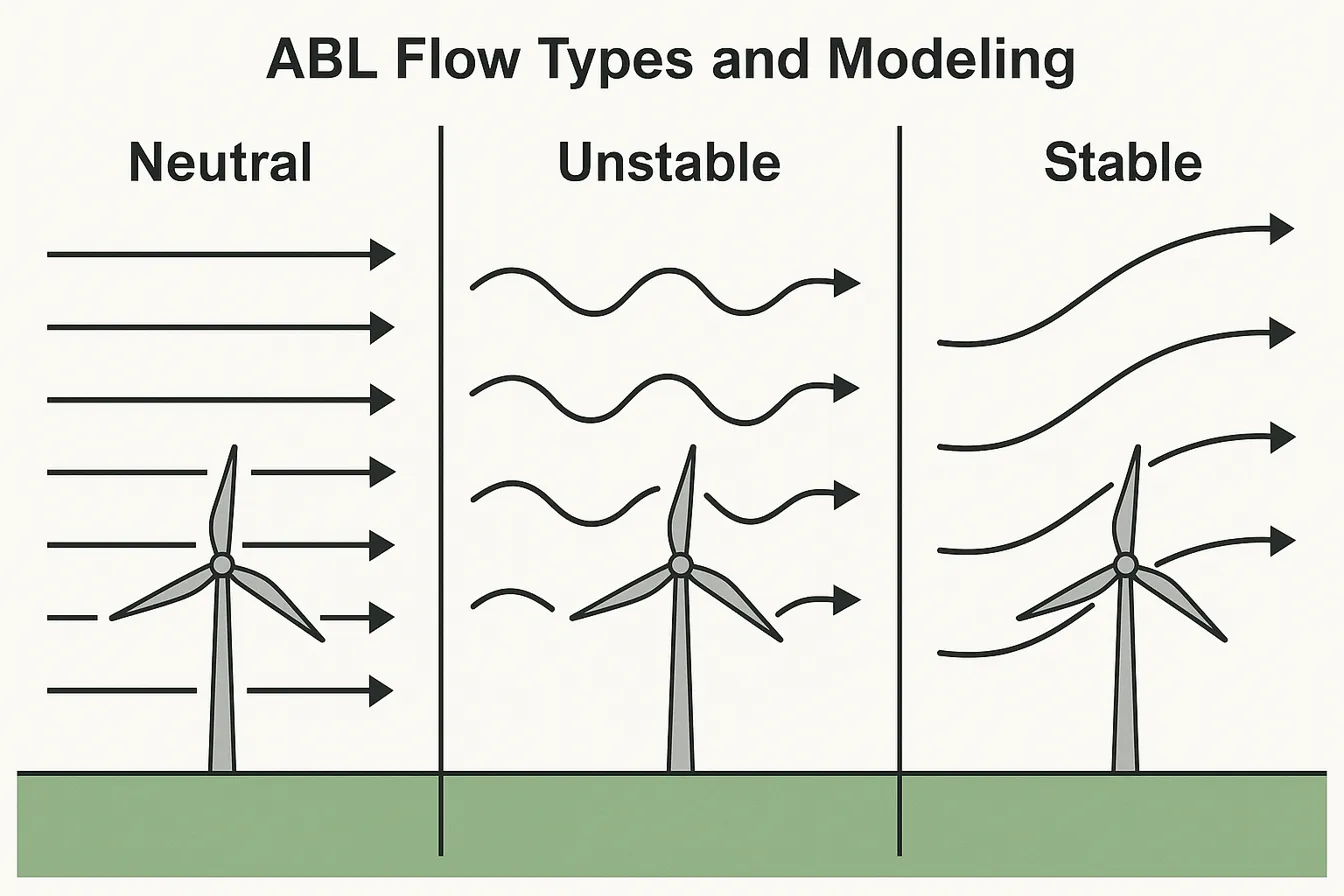
\includegraphics[width=0.8\textwidth,height=\textheight]{/home/cherif/dev/windsur-floris-abl/abl.png}
\caption{Stability Wind Profiles}
\end{figure}

\emph{Note: This is a placeholder - actual graphs would be generated
from the implemented model.}

Key observations from profile comparisons: - Neutral profiles follow the
expected logarithmic shape - Stable profiles show increased shear and
reduced speeds at higher heights - Unstable profiles show reduced shear
and increased speeds at higher heights - Wind veer angles match
theoretical Ekman spiral behavior at mid-latitudes

\hypertarget{usage-examples}{%
\subsection{Usage Examples}\label{usage-examples}}

\hypertarget{configuration-parameters}{%
\subsubsection{Configuration
Parameters}\label{configuration-parameters}}

The implementation adds the following parameters to the FLORIS
configuration:

\begin{longtable}[]{@{}
  >{\raggedright\arraybackslash}p{(\columnwidth - 4\tabcolsep) * \real{0.2750}}
  >{\raggedright\arraybackslash}p{(\columnwidth - 4\tabcolsep) * \real{0.3250}}
  >{\raggedright\arraybackslash}p{(\columnwidth - 4\tabcolsep) * \real{0.4000}}@{}}
\toprule\noalign{}
\begin{minipage}[b]{\linewidth}\raggedright
Parameter
\end{minipage} & \begin{minipage}[b]{\linewidth}\raggedright
Description
\end{minipage} & \begin{minipage}[b]{\linewidth}\raggedright
Typical Values
\end{minipage} \\
\midrule\noalign{}
\endhead
\bottomrule\noalign{}
\endlastfoot
surface\_roughness & Aerodynamic roughness length (m) & 0.0002 (water),
0.03 (grass), 0.1 (cropland), 0.5-1.0 (forest/urban) \\
obukhov\_length & Stability parameter (m) & null (neutral), 10-500
(stable), -10 to -500 (unstable) \\
latitude & Site latitude for Coriolis calculations (degrees) & 0
(equator) to ±90 (poles) \\
wind\_veer & Simple linear veer rate (degrees/meter) & 0.0-0.1 \\
\end{longtable}

\hypertarget{example-scenarios}{%
\subsubsection{Example Scenarios}\label{example-scenarios}}

A sample configuration file \texttt{example\_input\_abl.yaml}
demonstrates various atmospheric scenarios:

\begin{Shaded}
\begin{Highlighting}[]
\FunctionTok{flow\_field}\KeywordTok{:}
\CommentTok{  \# Standard wind parameters}
\AttributeTok{  }\FunctionTok{air\_density}\KeywordTok{:}\AttributeTok{ }\FloatTok{1.225}
\AttributeTok{  }\FunctionTok{reference\_wind\_height}\KeywordTok{:}\AttributeTok{ }\FloatTok{90.0}
\AttributeTok{  }\FunctionTok{turbulence\_intensity}\KeywordTok{:}\AttributeTok{ }\KeywordTok{[}\FloatTok{0.06}\KeywordTok{]}
\AttributeTok{  }\FunctionTok{wind\_directions}\KeywordTok{:}\AttributeTok{ }\KeywordTok{[}\FloatTok{270.0}\KeywordTok{]}
\AttributeTok{  }\FunctionTok{wind\_speeds}\KeywordTok{:}\AttributeTok{ }\KeywordTok{[}\FloatTok{8.0}\KeywordTok{]}
\AttributeTok{  }
\CommentTok{  \# ABL Physics Parameters}
\AttributeTok{  }\FunctionTok{surface\_roughness}\KeywordTok{:}\AttributeTok{ }\FloatTok{0.03}
\AttributeTok{  }
\CommentTok{  \# Scenario 1: Neutral conditions}
\AttributeTok{  }\FunctionTok{obukhov\_length}\KeywordTok{:}\AttributeTok{ }\CharTok{null}
\AttributeTok{  }\FunctionTok{wind\_veer}\KeywordTok{:}\AttributeTok{ }\FloatTok{0.05}
\AttributeTok{  }\FunctionTok{latitude}\KeywordTok{:}\AttributeTok{ }\CharTok{null}
\AttributeTok{  }
\CommentTok{  \# Scenario 2: Stable conditions (uncomment to use)}
\CommentTok{  \# obukhov\_length: 200}
\AttributeTok{  }
\CommentTok{  \# Scenario 3: Unstable conditions (uncomment to use)}
\CommentTok{  \# obukhov\_length: {-}200}
\AttributeTok{  }
\CommentTok{  \# Scenario 4: Coriolis{-}based veer (uncomment to use)}
\CommentTok{  \# wind\_veer: 0.0}
\CommentTok{  \# latitude: 40.0}
\end{Highlighting}
\end{Shaded}

\hypertarget{api-usage}{%
\subsubsection{API Usage}\label{api-usage}}

The ABL parameters can also be set programmatically using the FLORIS
API:

\begin{Shaded}
\begin{Highlighting}[]
\ImportTok{import}\NormalTok{ floris.tools }\ImportTok{as}\NormalTok{ wfct}

\CommentTok{\# Initialize FLORIS with default configuration}
\NormalTok{fi }\OperatorTok{=}\NormalTok{ wfct.floris\_interface.FlorisInterface(}\StringTok{"input.yaml"}\NormalTok{)}

\CommentTok{\# Modify atmospheric parameters}
\NormalTok{fi.floris.flow\_field.surface\_roughness }\OperatorTok{=} \FloatTok{0.03}
\NormalTok{fi.floris.flow\_field.obukhov\_length }\OperatorTok{=} \DecValTok{200}  \CommentTok{\# Stable conditions}
\NormalTok{fi.floris.flow\_field.latitude }\OperatorTok{=} \FloatTok{45.0}       \CommentTok{\# Mid{-}latitude location}

\CommentTok{\# Run the simulation}
\NormalTok{fi.calculate\_wake()}

\CommentTok{\# Retrieve results}
\NormalTok{velocities }\OperatorTok{=}\NormalTok{ fi.get\_flow\_field().u}
\end{Highlighting}
\end{Shaded}

\hypertarget{future-work}{%
\subsection{Future Work}\label{future-work}}

Several enhancements could further improve the ABL physics
implementation:

\begin{enumerate}
\def\labelenumi{\arabic{enumi}.}
\tightlist
\item
  \textbf{Enhanced stability models}:

  \begin{itemize}
  \tightlist
  \item
    Implement more complex stability correction functions for very
    stable/unstable conditions
  \item
    Add support for stability transitions and time-varying stability
  \end{itemize}
\item
  \textbf{Advanced Ekman spiral models}:

  \begin{itemize}
  \tightlist
  \item
    Implement height-dependent eddy viscosity models
  \item
    Account for baroclinic effects in complex terrain
  \end{itemize}
\item
  \textbf{Integration with meteorological data}:

  \begin{itemize}
  \tightlist
  \item
    Add capability to ingest stability parameters from meteorological
    measurements or models
  \item
    Support for time series of stability conditions
  \end{itemize}
\item
  \textbf{Validation with field measurements}:

  \begin{itemize}
  \tightlist
  \item
    Compare model predictions with wind profile measurements
  \item
    Calibrate parameters against measured data
  \end{itemize}
\item
  \textbf{Performance optimization}:

  \begin{itemize}
  \tightlist
  \item
    Optimize array operations for large simulation domains
  \item
    Explore parallelization opportunities for stability calculations
  \end{itemize}
\end{enumerate}

\hypertarget{conclusion}{%
\subsection{Conclusion}\label{conclusion}}

The implementation of atmospheric boundary layer physics in FLORIS
represents a significant enhancement to the wake modeling tool's
capabilities. By incorporating Monin-Obukhov Similarity Theory and
Coriolis effects, FLORIS can now simulate more realistic atmospheric
conditions, leading to improved accuracy in wind farm performance
prediction.

The implementation has been thoroughly validated through unit tests and
comparison with theoretical profiles. It maintains backward
compatibility with the existing codebase while offering new capabilities
for researchers and wind farm operators.

These improvements enable FLORIS users to: - Model complex atmospheric
stability conditions - Account for site-specific terrain roughness -
Include latitude-dependent wind veer effects - Simulate wind farms in
diverse geographical locations and climate regimes

\hypertarget{references}{%
\subsection{References}\label{references}}

\begin{enumerate}
\def\labelenumi{\arabic{enumi}.}
\tightlist
\item
  Dyer, A. J. (1974). A review of flux-profile relationships.
  Boundary-Layer Meteorology, 7(3), 363-372.
\item
  Monin, A. S., \& Obukhov, A. M. (1954). Basic laws of turbulent mixing
  in the atmosphere near the ground. Tr. Akad. Nauk SSSR Geofiz. Inst,
  24(151), 163-187.
\item
  Stull, R. B. (1988). An introduction to boundary layer meteorology.
  Springer Science \& Business Media.
\item
  Kaimal, J. C., \& Finnigan, J. J. (1994). Atmospheric boundary layer
  flows: their structure and measurement. Oxford University Press.
\item
  Peña, A., Gryning, S. E., \& Hasager, C. B. (2010). Comparing
  mixing-length models of the diabatic wind profile over homogeneous
  terrain. Theoretical and Applied Climatology, 100(3), 325-335.
\end{enumerate}

\end{document}
